\documentclass{article}
\usepackage{amsmath}
\usepackage{graphicx}
\begin{document}
\section{Execute}
\subsection{Circuit Diagram}
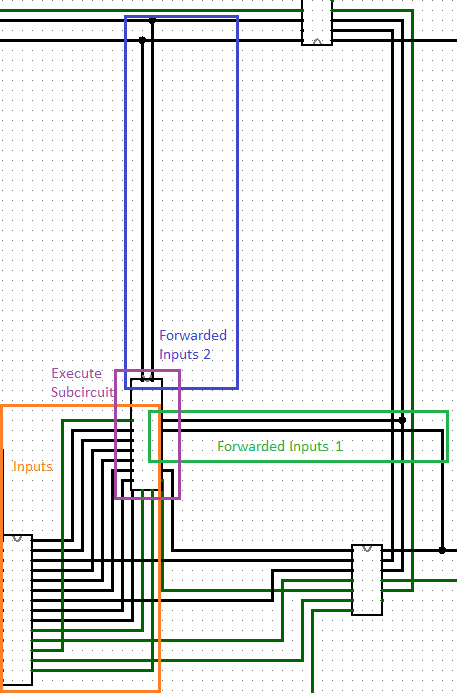
\includegraphics[width=8cm]{ALU.png}
\\
Our Execute stage is all condensed into a big Execute subcircuit, that does the computing, (with additional lower level circuits within the subcircuit) and a smaller subcircuit that aids in stalling. The Execute subcircuit gets its inputs mainly from the ID/EX registers but also from the EX/MEM and MEM/WB registers for use in the forwarding unit. The four outputs of the subcircuit is the main output C, the Write Enable for the Register File (which is conditional in the MOV instructions), a Jump variable, indicating whether or not we branch, and an output for Store functions. 

The Execute subcircuit has many subcircuits of its own. For each of the main inputs, A and B, with respective register addresses rs and rt, there is a forwarding unit that resolves data hazard issues that are present in this Mini-Mips processor. There is a multiplexor for B that chooses between B and the immediate. There are special sections that implement commands whose outputs do not come from the ALU. These commands include SLT, SLTI, SLTIU, and SLTU; MOVZ and MOVN; jumps and branches; and SW and SB. 

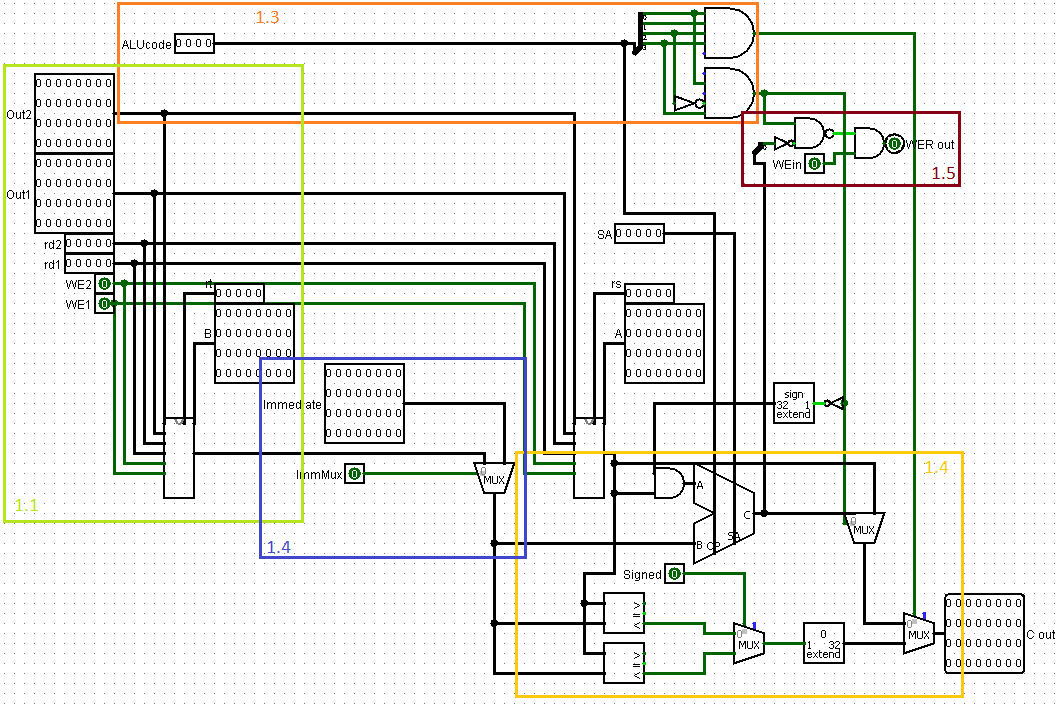
\includegraphics[width=17cm]{EXOVER.png}

\subsubsection{General Purpose ALU}
The ALU (1.3) provides us the output for many of the simpler commands, and also provides us some intermediate outputs for the more specialized commands. Inputs A and B are determined by the specified command, but here we take them as given. We get the Op Code for the ALU as an input (1.1), and the SA is determined in a subcircuit (1.2), depending on whether or not the shift command was variable.  

\subsubsection{Forwarding Unit}
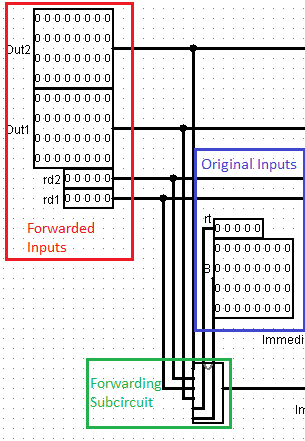
\includegraphics{Forward1.png}
This part of the circuit compares the register address (rs) of a main input (Out0) with the write destinations of the instruction in the next stage (rd1) and the stage after that (rd2). Out1 and Out2 are to be written in those destinations respectively. The write enable bits from those stages need to be included as well. The Forwarding Unit takes these 8 inputs and chooses one of the 3 32-bit outputs Out0, Out1, Out2. Figure 11 shows the layout of the Forwarding Unit and its inputs in the Execute circuit.

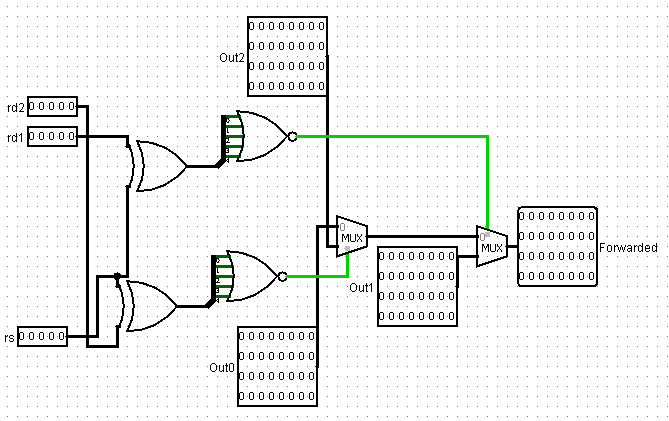
\includegraphics{Forward2.png}
The Forwarding Unit compares the register addresses using an XOR and a NOR gate to get a multiplexor selector, that is, if the register addresses are equal, we get 1, and otherwise 0. Additionally, the current register address must not be 00000. This is ANDed with a write enable bit. This is done for each rs and rd1, and rs and rd2. We first choose between Out0 and Out2 by comparing rs and rd2, then the selected and Out1 by comparing rs and rd1. This process automatically gives Out1 higher priority than Out2; if all of rs, rd1, and rd2 are equal, Out1 will be chosen over Out2. 

Load Forward (2.3) simply computes whether the previous instruction's register address (rd) is the same as the current instruction's rs or rt. This output is used later on in stalling for LW forwarding.

\subsubsection{Immediate Mux}
This section (3.1) determines which of input B or the Immediate become an input for the ALU and the Comparators.

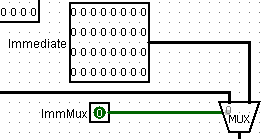
\includegraphics{Immediate.png}
The upper MUX determines the second input of the ALU. The Immediate is already bit extended to 32 bits, and our Decoder gives us a multiplexor selector bit ImmMux that we use here. 

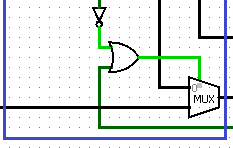
\includegraphics{Immediate2.png}
The lower MUX determines the second input of the Comparators. The difference between this MUX and the upper MUX is that the MUX will choose input B if the command is a Branch command, overriding the ImmMux. 

\subsubsection{MOVN/MOVZ}
MOVN and MOVZ are one of the sets of commands that require special attention. The large AND gate in (4.1) outputs 1 if the ALU Op code is 1x01. Directly right of the AND gate is a subcomponent that disables the Register Write Enable if the ALU returns 0 for the comparison. 

The AND gate in (4.3) replaces input A with a 32-bits of all 0's if the command is MOVN or MOVZ. This is because these commands' conditionals compare against zero. 

Finally the output that is eventually stored if the conditional is true is the input A. Our MUX in (4.2) does exactly that, choosing input A over the ALU output C if the selector bit is 1.

\subsubsection{Comparator}
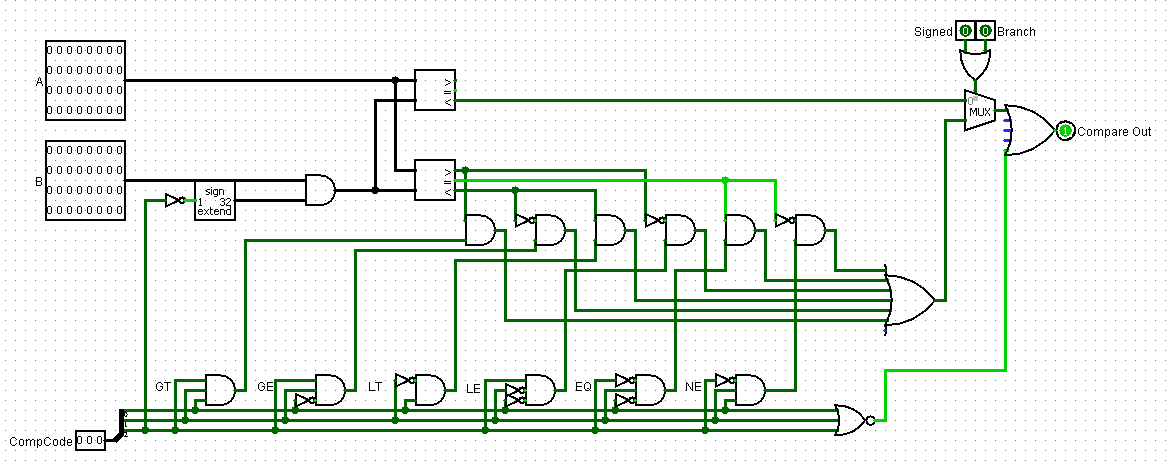
\includegraphics{Compare.png}
The Comparators (5.3) is used for the SLT commands and the branch commands. The upper comparator is unsigned and used for the commands SLTU and SLTIU. 

We use a Comp Code that tells us the exact comparison that we want. 

\begin{tabular}{| c | c |}
\hline 
LEZ & 100 \\ \hline
LTZ & 101 \\ \hline
GEZ & 110 \\ \hline
GTZ & 111 \\ \hline
SLT & 001 \\ \hline
EQ &  010 \\ \hline
NE &  011 \\ \hline
\end{tabular}

\textbf{Design Decisions}
\begin{itemize}
\item
We set all the Comp Codes for comparisons with 0 to 1xx, so we sign extend the negation of the most significant bit of the Comp Code to control the second input to the comparators. 
\item
We represent GE and LE as the negation of LT and GT respectively and that can be seen in the first row of AND gates under the second comparator.
\item
Only 1 of the outputs from the second row of AND gates is 1 for any Comp Code. That means only 1 of the outputs from the first row of AND gates can be 1, and the big OR gate will output 0 unless that specified comparison is true. 
\item
The Comp Code for all other commands is 000, which makes the output of the subcircuit 1 regardless of the inputs. This is required so that Jump instructions always jump.(see (6.3))
\end{itemize}

Back in the Execute circuit, the Op code 1111 identifies the command as one of the SLT commands, and the MUX in (5.2) and the selector bit in (5.1) choose the zero extended Comparator output to be the final output. 

\subsubsection{Jump and Branch}
Jumps and Branches also require special computing. 

The branch conditionals are done in the Comparator (see above) which then turns off or maintains the Jump variable in (6.3). The target address for a branch is computed in the ALU. The PC in (6.1) is incremented by 4 and then chosen for in the MUX in (6.2) to be the first input of the ALU. 

The target address for a jump is computed in a separate subcircuit, which is done simply by using splitters. 
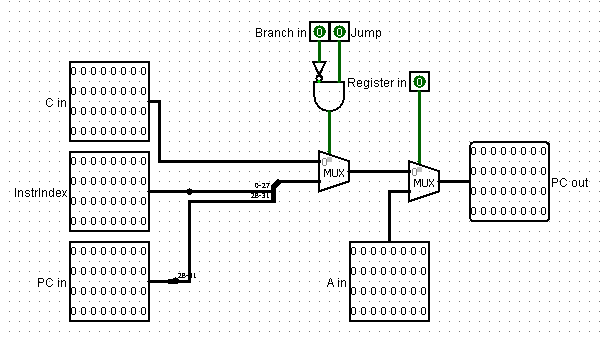
\includegraphics{Jump.png}

The subcircuit also chooses between the jump target address and the branch target address and address stored in a register depending on the related bits. 

\subsubsection{Store Output}
In (7.1), we simply output the input B which is stored in RAM in the instructions SW and SB.

\subsubsection{LoadStall Disable}
This small subcircuit in the main circuit simply disable the Jump variable, Load Enable, Register File Write Enable, and RAM Write Enable in the Execute stage during a stall. These 4 variables when all disabled effectively prevent the instruction from doing anything.

\subsection{Correctness Constraints}
\begin{itemize}
\item The correctness of this module depends on the correctness of the inputs that are decoded in the Instruction Decode stage. Therefore, one functional requirement is that the inputs are consistent with the MIPS command given. For instance, WE in (write enable) must be 1 if the command ultimately writes back to the Register File. 
\item The module takes inputs from the Memory and Write Back Stages. Therefore, these stages need to be implemented correctly in order for this stage to be correct.
\item The execute subcircuit in this implementation is only correct for the instructions in Table A and Table B. Only these instructions can be given in the Instruction Fetch Stage.
\item There are also certain limitations on the ordering of instructions given, namely that a Jump or Branch cannot be given in the delay slot of another Jump or Branch. However this is a limitation on the whole circuit, not on the Execute stage itself.

\end{itemize}

\subsection{Testing}
A large portion of the instructions depend on the correctness of the ALU circuit. Since that is given to us, we assume its correctness. For those instructions, computation is given correct, so we only have to test one case for each, that is, if one case gives us the correct nontrivial output (like 0 or something that could have been an accident), then the data path was correct and all inputs for that instruction should give us a correct output. 

For the function that are not computed solely using the ALU, we need to check an encompassing set of cases. Many of the Table B instructions' correctnesses are not solely dependent on the execute stage, but the overall testing for those instructions will be mentioned here. Load and Store will be elaborated more in Memory.

For the SLT, MOV, and Branch instructions, we check all the cases for the conditionals, namely less than, greater than, and equal. For branches we need to check if the delay slot works properly and if the instruction after the delay slot is canceled properly. We also check if branching with both negative and positive offsets work properly.

For the Jump instructions, we check if the delay slot works properly and if the instruction after the delay slot is canceled properly, as in the Branch tests. The register Jumps also need to be tested, and we have to check if the link address is stored properly in JAL and JRAL. 

Load and Store only have their addresses computed in the ALU in the Execute stage, which is trivial. The bulk of their correctness is dependent on the Memory stage.

Lastly, we need to test the forwarding unit. We need to test for EX/MEM $\rightarrow$ EX forwarding and MEM/WB $\rightarrow$ EX forwarding. We test with multiple cases to be safe. 

\section{Memory}
\subsection{Circuit Diagram}
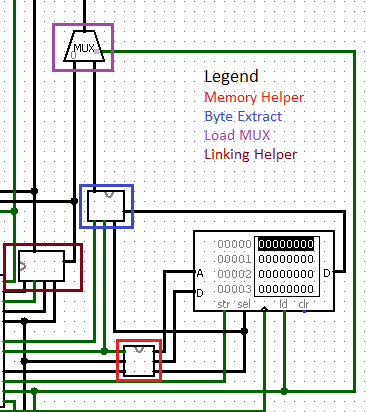
\includegraphics[width=8cm]{MemOver.png}

Our Memory stage has 3 main subcircuits:

 The Memory Helper processes the outputs from the Execute stage to give us the Byte Selector, the 20 bit Memory Address, and the RAM input. 
 
 The Byte Extract, much as the name suggests, extracts the byte from RAM output in LB and LBU instructions, and does nothing otherwise.
 
 The Linking Helper processes outputs from the Execute stage to set rd to 31 and choose the address to be written. 
 
 There is also a MUX that chooses for the RAM output if the Load Enable is on.
 
\subsubsection{Memory Helper}
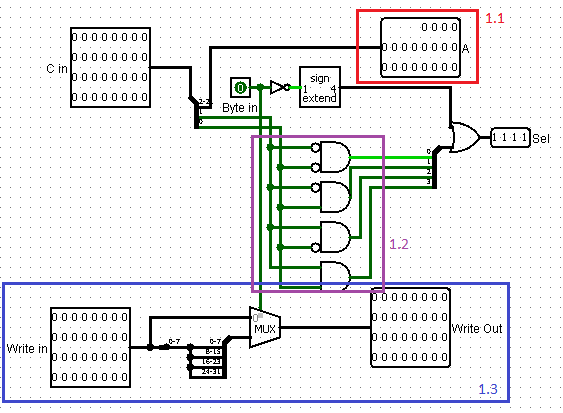
\includegraphics{MemHelp.png}
The first output in the Memory Helper is the Write Address A (1.1). This is acquired by simply extracting bits 2-21 from the main Execute output C. 

The second output is the RAM input (1.3). This is either the original Write in if the instruction is SW or its first byte replicated 4 times if the instruction is SB. ("Byte in" indicated whether the memory instruction is Word(0) or Byte (1)) 

The final output is the Byte Select. The AND gates in (1.2) extract from the first 2 bits of "C in" the Byte information. Only one of the AND gates can output 1 at a time, so our Byte Select is for the most part limited to one of 0001, 0010, 0100, and 1000, which is what we want. The exception to this rule is when the instruction isn't a Byte instruction, in which case the Byte Select is 1111, which we get by using an OR gate with the negation of "Byte in", sign extended. 

\subsubsection{Byte Extract}
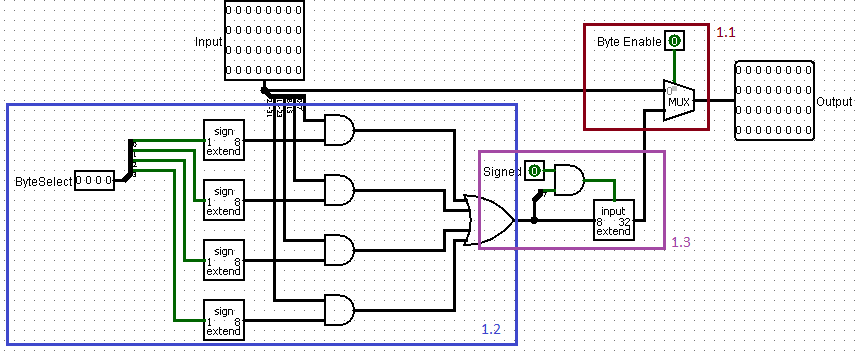
\includegraphics{ByteExtract.png} 
 The Byte Extract, much as the name suggests, extracts the byte from RAM output in LB and LBU instructions, and does nothing otherwise.
 
 From the MUX in (1.1), the 

\end{document}